This section aims to present the reader with basic information, and knowledge, needed to understand the rest of the thesis. 
The goal of the thesis is to tackle two different problems: improving land cover classification maps based on SAR images, and improving 
change detection algorithms based on SAR Images. 
Therefore, it is important that the reader be familiarized with three topics - that will be introduced in this chapter - which we will dwell upon to build this material: SAR images, Land cover Maps and
change detection algorithms.

\section{Principles of Wavelenght-Resolution SAR Systems}
Remote Sensing (RS) is the science of extracting information about an object, without using sensors in physical contact with the said object. Remote sensing has applications in several fields, including geology, meteorology, hydrology, ecology, land surveying, among others \cite{survey-rs}. Currently, "remote sensing" generally refers to the use of satellite or aircraft-based sensors to detect and classify objects in the Earth. Moreover, these sensors can be of two types: passive sensors (when the sensor detects the reflection of sunlight) or active sensors (when the sensor emits its own signal and detects the reflection of the emitted signal).

This work will focus on a specific type of sensor, the Synthetic Aperture Radar (SAR).
SAR is a side looking radar used in remote sensing for imaging purposes. It consists of an antenna that sequentially transmits electromagnetic waves to the Earth's surface, and registers the reflection of these transmitted waves. Through signal processing techniques, it is possible to coherently combine the received echoes registered by the SAR, making possible to create a reflectivity scene of the area. On top of that, the coherent combination of the echoes also makes possible to record amplitude and phase of the received signal. For a more detailed explanation regarding SAR it is recommended \cite{livro}.

Figure \ref{fig:SAR_geometry} presents the basic geometry concerning the workings of a SAR system. The flight direction is called azimuth direction, and the $x$ axis is called "across-track" direction, or ground range direction. The "slant-range" direction is the direction of the line that connects the object on the ground, and the sensor.

\begin{figure}[H]
    \centering
    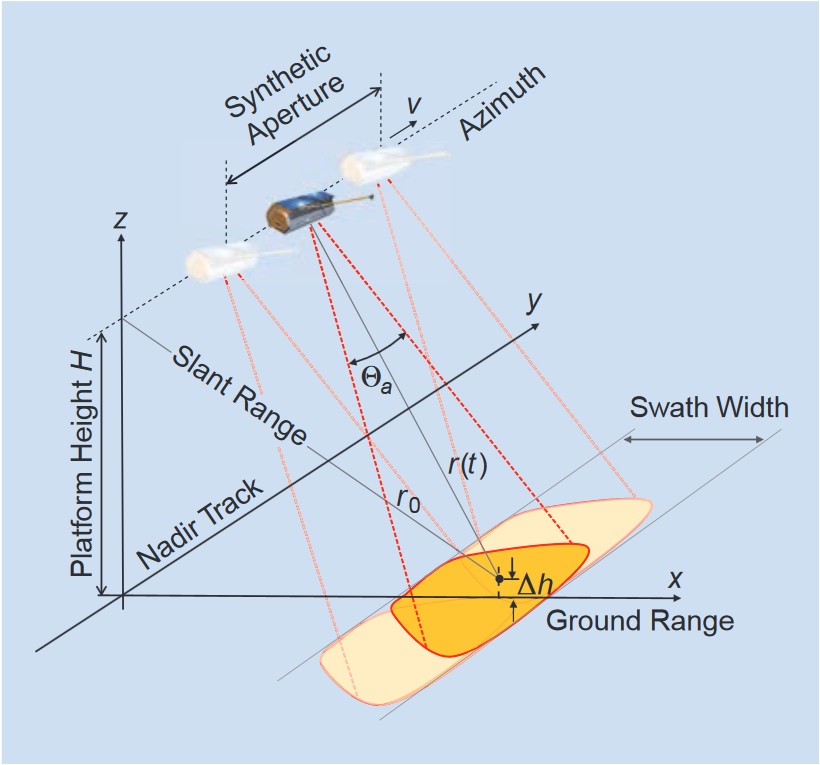
\includegraphics[width=0.8\linewidth]{Cap1-Bib Review/geometry.png}
    \caption{Illustration of SAR geometry. $r_0$ is the shortest distance to target, $\theta_a$ stands for the azimuth beam width and $v$ for the satellite speed. \cite{tutorial}}
    \label{fig:SAR_geometry}
\end{figure}{}

The resolution of a SAR system is the minimal distance that makes possible to detect two objects as separate objects in the image (for any distance below the resolution two objects will appear as a single object for the observer). In SAR systems, the resolution is not unique, since the system can have different resolutions in the range direction and in the azimuth direction. 

For SAR systems, the resolution in azimuth direction is equal to half the antenna length, and the resolution in range direction can be calculated by \cite{62}:

\begin{equation}
    \delta = \frac{\lambda_c c}{4 \theta_H B}
\end{equation}
where $\lambda_c$ is the wavelength corresponding to the radar central frequency, $\theta_H$
is the aperture angle (in radians), $c$ is the speed of light and $B$ is the system bandwidth.

Wavelenght-Resolution SAR systems, are radar systems with resolution in the order of the system wavelength. The SAR systems used throughout this work are wavelength-resolution SARs, so some facts concerning these systems must be mentioned. 

When using wavelength-resolution SARs to detect targets, it is important to mention that the size of the target matters to the final image registered. According to \cite{63}, SAR images of targets with dimensions of the order of the Wavelength might present the resonance scattering phenomena \cite{63}, and targets small compared to the wavelength might present the Rayleigh scattering phenomena\cite{63}. 

Another major cause of problems in SAR images is the Speckle noise. According to \cite{63, 17}, speckle noise is mainly due to multiple targets reflecting the emitted pulses, but since for Wavelenght-Resolution SAR, the target's size are approximately the order of the wavelength - and therefore, close to the system resolution - there can be only one scatterer inside each resolution cell, so for target detection using wavelength-resolution SAR, speckle is not a main cause of problems. Because of that it is of great importance to choose an appropriate frequency when designing the SAR system, since different system frequencies will be more, or less adequate, for detecting targets of different sizes. 

\subsection{SAR Images}
After registering the received echoes, it is still necessary to perform image processing techniques, since the image is not yet ready for interpretation and information extraction\cite{Alberto}. The first step of the process is to perform matched filter operations to enhance the received signal, this is done by doing convolutions of the received images with the reference signal in the azimuth direction and the range direction. For more details concerning the convolution process the reader it is referred to \cite{Alberto, livro}.

After performing the relevant convolutions, it is obtained a complex image (with amplitude and phase information) that is called Single Look Complex (SLC) matrix. The amplitude value of this image represents the power reflected back to the antenna. The backscatter -  value that is analogous to reflectivity - of the scene can be obtained by multiplying the amplitude value by a calibration constant obtained experimentally.
The backscatter alone is of great importance to the interpretation of the image, since it alone can suffice to detect and classify objects on Earth's surface \cite{radiometric}, since different objects will present different backscatter characteristics.

According to \cite{Raney,Small} it is also possible to define different backscatter measures. The backscatter value represents the reflectivity (normalized by the area of incidence), which can be measured in different directions. The backscatter previously mentioned is the reflectivity value measured in the range direction (which has area $A_\beta$), and it is called beta-naught($\beta^0$). It is also possible to measure reflectivity in the ground direction(which has area $A_\gamma$) - reflectivity value which is called gamma-naught ($\gamma^0$) - and in the direction perpendicular to the range direction (which has area $A_\sigma$) - reflectivity value which is called sigma-naught ($\sigma^0$). All these values are of importance, since they all can be used to characterize the scene and be used to perform target detection and classification. 

The relationship between $\gamma^0$ and $\beta^0$ can be obtained by the formula $\gamma^0 = \beta^0 \cdot \sin(\theta)$ and the relationship between $\sigma^0$ and $\beta^0$ can be obtained by the formula $\sigma^0 = \beta^0 \cdot \tan(\theta)$, where $\theta$ is the incidence angle of the emitted pulse.

A visual description of these normalized backscatter coefficients is shown in \figref{fig:normalization_areas}

\begin{figure}[H]
    \centering
    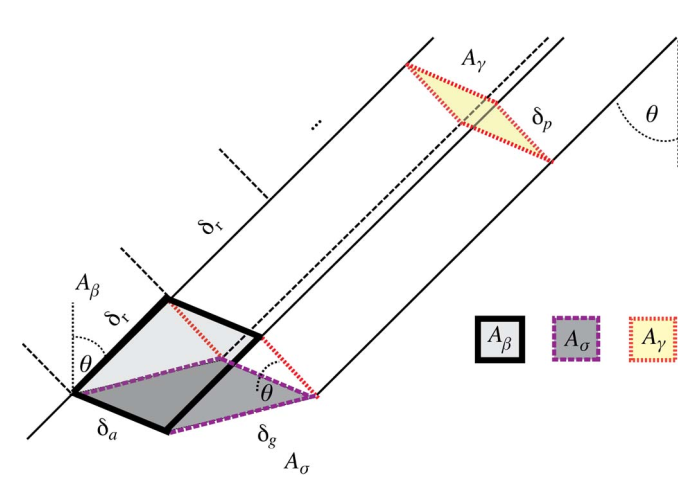
\includegraphics[width=0.8\linewidth]{Cap1-Bib Review/retang.png}
    \caption{Normalization areas for SAR backscatter. \cite{Small}}
    \label{fig:normalization_areas}
\end{figure}

After obtaining the SLC image, it is also necessary to perform additional steps for obtaining an image that is ready for visual interpretation, such as, coregistration, geocoding, calibration, among others steps. These steps are outside the scope of this work, for the curious reader it is referred \cite{Alberto} for more details concerning these image processing techniques.

\subsection{The Coherence Image}
After performing all necessary steps the final SLC image obtained is ready for visual interpretation. This SLC image alone is enough to provide results for classifying and detecting objects, and scenarios, on the Earth's surface, as it can be seen in \cite{Paolathesis,Andreathesis, 78, 79, rfsar}, but there are techniques that make possible to extract information based on combining different SLC acquisitions.

When two images of the same area are collected, it is possible to combine both images into a single image named the "interferometric coherence image". The coherence image can be calculated by taking the complex correlation between the pairs of corresponding pixels of the two acquisitions, and it is calculated as:

\begin{equation}
    \gamma = \frac{E[u_1u_2^*]}{\sqrt{E[|u_1|^2]E[|u_2|^2]}}
\end{equation}{}

where $E[\cdot]$ is the expectation operator, $u_1$ is a pixel of the first image and $u_2$ is the corresponding pixel on the second image. One must keep in mind that it is not possible to compute the expected value since the probability density function (PDF) for the pixel is not known, so in practice the correlation is computed using numerical estimations around the pixel of interest. For more details concerning the numerical estimation - and the trade-offs between computing methods - of the complex coherence, the reader is referred to \cite{Bamler}. 

After extracting the complex coherence (some sources use the term correlation/decorrelation instead of coherence) between pairs of images, the final result is an image that provides relevant information for classification and target identifying purposes as it can be seen in \cite{Alberto,Paolathesis,Martone, Martone2, Martone3, first_interferometric, Krieger,Paolo, Acqua} among others.

There are multiple factors that can affect the final coherence image, some of which are irrelevant for this work, and some of which are very relevant for the final result of this work. In \cite{Krieger,Paolathesis} there is a detailed explanation concerning the coherence factors, but for this work purpose only two coherence factors matter:
\begin{enumerate}
    \item $\gamma_{Temp}$: Is the coherence factor due to the temporal baseline between both acquisitions. The longer the acquisition between the two images, the more degraded the final coherence image will be due to this temporal coherence factor.
    \item
    $\gamma_{Vol}$: is the volume correlation factor, and it is due to volume scattering (scattering caused by multiple scatters inside the same resolution cell). On forests this is mainly due to vegetation and therefore is crucial for forest land-cover classification.
\end{enumerate} 

The temporal and volumetric coherence are crucial for the creation of land cover classification maps, as it can be seen in \cite{Paolo, Rodrigo}, so the reader is referred to these works to better understand the applications and models used for the creation of land cover maps from coherence images.

\section{SAR Images for Land Cover Classification Maps}

Land Cover maps are maps that measure the area and perimeter of different field types on the Earth's surface. Since land coverage maps have broad applications - ranging from environmental, economical and ecological purposes - it is important that the accuracy be as high as possible. Since it is not feasible to physically measure the environmental degradation of a forest (because this does not scale well to large areas), normally these measurements are done with remote sensing data. The GlobCover \cite{globcover, glob} (European Space Agency GlobCover Portal) map is one example of a classification map that was generated using MERIS data.

When dealing with coverage maps, there are mainly three areas of interest: vegetated areas, deforested areas, and artificial surfaces (human made surfaces like constructions, buildings, roads, houses, etc...). Among these areas, they can be further divided in subclasses, for example, vegetated areas can be further divided between:irrigated croplands, deciduous forests, mosaic grassland among others. This is the standard used by the GlobCover map (and many others land coverage maps) and can be seen in Figure \ref{fig:glob_cover_map}.

\begin{figure}[H]
    \centering
    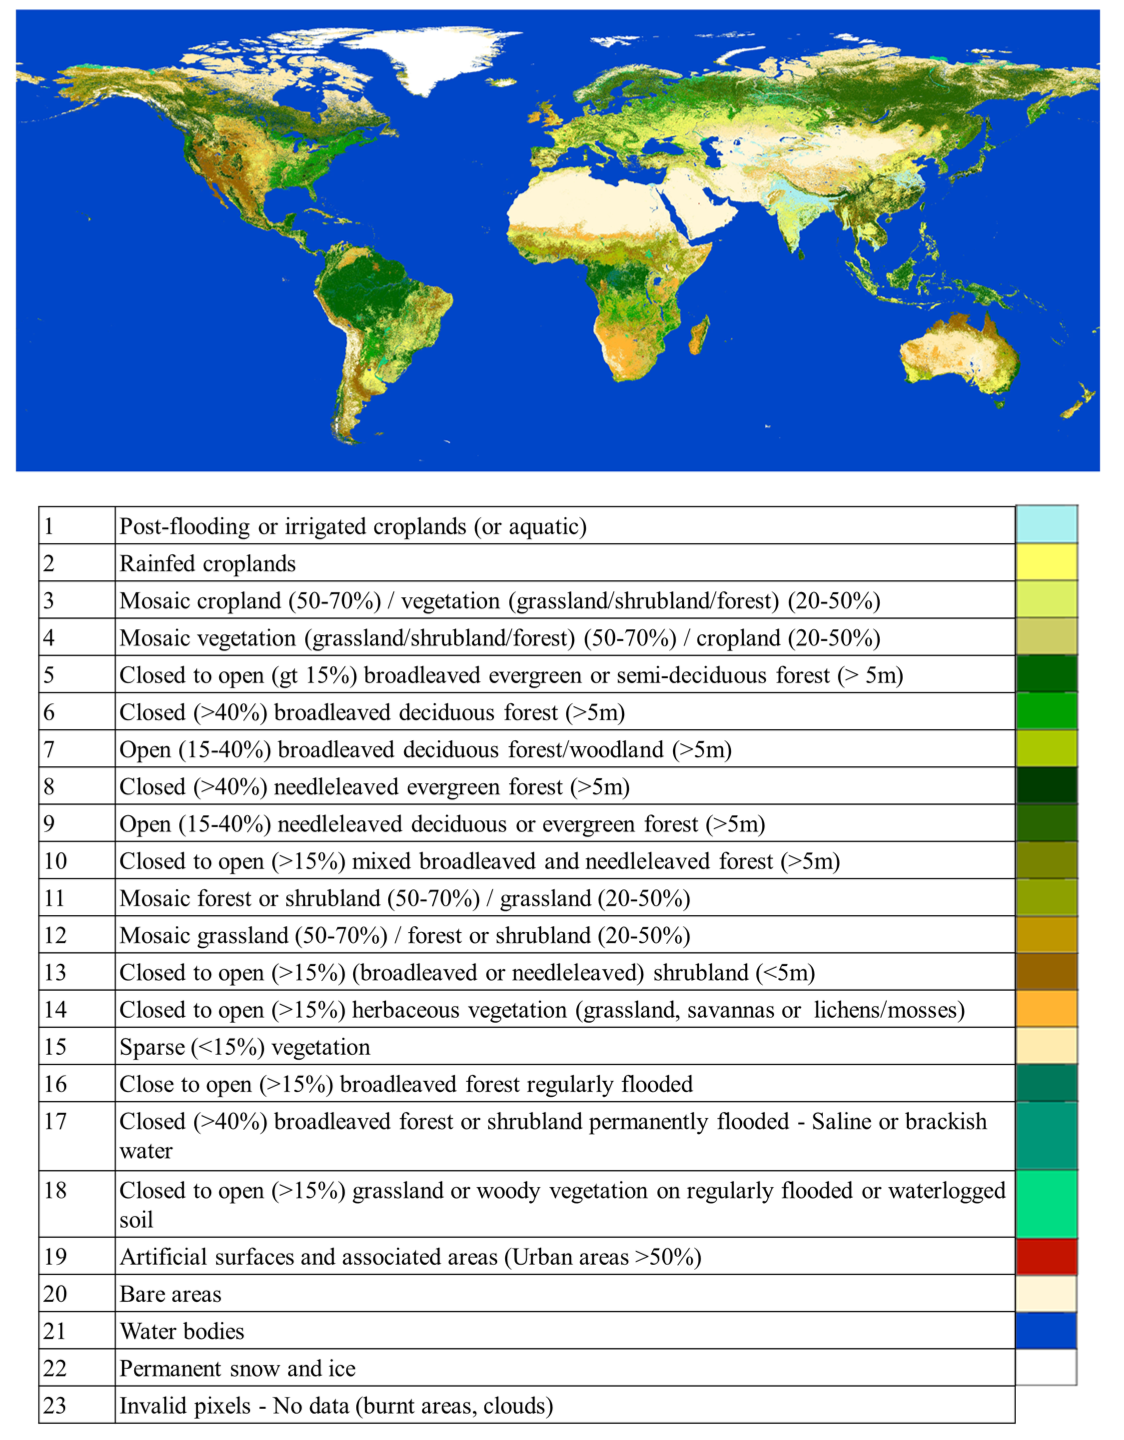
\includegraphics[width=\linewidth]{Cap2/glob_cover.png}
    \caption{GlobCover classification map \cite{Paolathesis}.}
    \label{fig:glob_cover_map}
\end{figure}

GlobCover map was created using optical sensors instead of laser sensors. This method has the advantage that it is easy to create a classification from its data, but it has the disadvantage that it is weather dependent and cannot provide a high resolution map.
SAR land coverage maps have none of these disadvantages, but it comes at the price that it is harder to create an accurate classification map.

The L-Band ALOS PALSAR \cite{alos1, alos2, alos3,alos4, alos5, alos6} is a global coverage map created from SAR acquisitions based only on creating thresholds on the cross-polarization levels of the detected backscatter. Using ALOS PALSAR data, several forest maps were created for the Amazon rainforest - and other tropical forests -  that present very high classification accuracy, therefore it is used for practical purposes.

Even though it is possible to create land coverage maps based only on the backscatter measurement, it is possible to use the coherence information to further improve the accuracy results. \cite{first_interferometric} was the first reported case of forest coverage map created using coherence information. This work was done using ERS-1 SAR data and proved that not only forests can be clearly discriminated from other land categories, but it also showed that it is possible to distinguish among different forests types. By analyzing statistical properties of the coherence values of the area (such as mean and standard deviation) it was possible to infer which class that specific pixel belongs to. In \figref{fig:first_interferometric_estimate} it can be seen the statistical properties of coherence for different classes.

\begin{figure}[H]
    \centering
    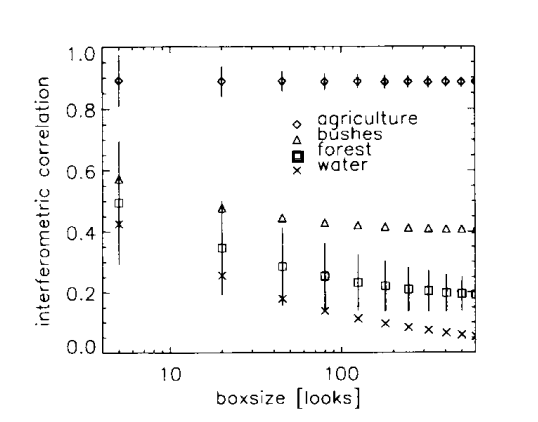
\includegraphics[width=0.7\linewidth]{Cap2/first_interferometric.png}
    \caption{Mean and Standard deviation of the coherence estimate as number of looks (filter size) for different classes.}
    \label{fig:first_interferometric_estimate}
\end{figure}

Throughout this thesis, both techniques were combined in order to improve the accuracy of the land cover classification maps. The backscatter information will be combined with the coherence information to try to achieve a maximum accuracy land coverage map. The work was based on other works that try to do a similar approach to solve this problem, such as the works in \cite{Paolathesis,Paolo, Martone, Martone2, Martone3, Rizzoli}. The work will also propose new approaches to improve the statistical analysis of the values for backscatter and coherence, similar to what was done in \cite{first_interferometric}, but with more significant results due to better computational power that is available today. This method is also very detailed in a publication derived from this thesis and can be seen in \cite{Rodrigo}.

\section{SAR Images for Change Detection Algorithms}
When working with SAR systems, it might happen that multi-temporal acquisitions of the same area are performed, i.e., acquisitions of the same geographical area obtained with a temporal baseline between them. These multi-temporal images can be used for information extraction in two different manners: one way is to assess the information contained in the entire time frame, and the other way is to assess the difference that has occurred between images\cite{change1}. Change detection in remotely sensed data may be done in a supervised or an unsupervised way. Supervised techniques requires that a ground truth be available in order to derive a training set for the training process of the detectors, meanwhile unsupervised techniques do not have the requirement for ground truth data\cite{change2,change3}. Since the creation of ground truths is a very time demanding task, normally unsupervised change detection algorithms are performed, but normally they come with the disadvantage that unsupervised algorithms underperform when compared to supervised algorithms.

Change detection problems can be seen as a special case of multi-temporal images classification problems. Normally change detection algorithms work with two approaches: pre-classification approach and post-classification approach. Pre-classification approaches work by independently classifying the relevant pair of images and then an algorithm is used to identify the pixel labels that have changed. In the post-classification approach, a single classification is performed directly on the combined image dataset for the image pairs\cite{change4}. On this work, it will be proposed a new technique that is a mix of the pre-classification approach and the post-classification approach.

Even though there are multiple approaches and algorithms for change detection, most of them dwell on two problems\cite{change5}:
\begin{enumerate}
    \item Creating a change measure or change indicator image
    \item Thresholding the change indicator values to produce a binary change map.
\end{enumerate}

There are several measures that can be used to detect change, normally the change measure used is based on the ratio, or the log-ratio of the two images\cite{change6}, but there are plenty other measures that can be used as change measure, e.g., mean-ratio operator, triplet Markov field model measure, Radon transform, Jeffrey divergence, Garbor functions, power spectrum of the image, among others \cite{change5, change6, change7}. Even though most of the change measures are related to the post-processed and filtered image, there are techniques that rely on the noise, and speckle of the image: one prominent approach, that shows high accuracy, is based on modelling the speckle of the image as a fractional brownian motion and as a fractal image, extracting information concerning the brownian motion and the fractal dimension of the image and using this value to create the change measure for classification \cite{change5}. 

After the creation of the change measure, the only step left is to create the change detection algorithm based on the change indicator image. Traditional CDAs are based on standard statistical theory, e.g., traditional hypothesis testing criterion methods, such as generalized likelihood ratio test \cite{GLRT1,GLRT2,GLRT3}, 
maximum a posteriori criterion \cite{Book_Kay},
Bayesian theory approaches \cite{Bayes1, Bayes2},
or likelihood ratio test \cite{LRT1,LRT2,LRT3}. Most of these methods perform adequately in terms of probability of detection, but most show poor performance in terms of false alarm rate \cite{Carabas,Ricardo,LucasRamos,Chris}. Those methods also have few other drawbacks, such as dependency on additional preprocessing of the images throughout morphological operations (erosion and dilation filters) and the calibration of the algorithm before its use.

By trying to overcome the limitations of traditional statistical-based CDAs, machine learning algorithms became popular in the last few years \cite{Vinholi, Campos} since they can perform better than statistical-based CDAs and do not have the drawbacks that those methods present. There are two kinds of machine learning algorithms: supervised and unsupervised algorithms. Supervised algorithms are the ones that have a classification reference to help guide the learning step, while unsupervised algorithms are those that do not have the classification reference. In this dissertation, we focused only on supervised algorithms. As mentioned earlier, it is important to know the parameters of interest to quantify the quality of the algorithm under analysis. In other words, we can assess performance based on the number of true positives, true negatives, false positives, and false negatives \cite{PefMe}. From now on, the parameters of interest are the number of true positives and false negatives.

Among the supervised machine learning algorithms, there are many options for the applications considered in this dissertation, such as Neural Networks, Naive Bayes, Linear Regression, Kernel Ridge Regression, Support Vector Machine, Decision Trees, Random Forest \cite{PefMe}.
For this work, it is used neural network-based algorithm for the CD problem. There are multiple types of neural networks, e.g., perceptron, Feed Forward Neural Network, Multilayer Perceptron, Recurrent Neural Network, Long Short-Term Memory Neural Network, convolutional neural network, among others \cite{PefMe}. We decided to use a UNET convolutional neural network \cite{Unet}, to solve the target detection problem since CNNs have provided excellent results for computer vision problems. In \cite{Kevin} a similar approach was used to detect changes in SAR images, although the SAR images were acquired in a higher frequency band.

Generally, the priority of CDA designs is to maximize the percentage of true positives keeping as low as possible the false positives. This is relevant in many applications, such as detecting hidden objects over a large area, where a small number of false positives is vital in the quality of the final data for operation application - which is the main concern of this work. For this work, the approach chosen for the classification method will be a UNET CNN based network for the creation of the final change detection map. The UNET CNN uses SAR images as input for the target detection, but also textural information is explored according to the method. In \cite{Rodrigo}, it was already shown that additional textural information could provide valuable information to improve classification results. It is important to mention that since CNN uses convolutions, which are linear filters, to achieve better classification results, it would be redundant to use linear textural information as inputs to the UNET CNN. When comparing the proposed technique with other algorithms on the same dataset, we show that the results show similar detection performance but significant improvement in false alarm rate.